\section{Desarrollo} \label{sect:desarrollo}

Durante esta fase se implementó progresivamente la versión alfa de una aplicación móvil y servidor web, para dar solución al problema de registro y control de gastos. 

Para cumplir con los requerimientos del componente móvil, se creó una aplicación para el sistema operativo Android, y se trabajó con el IDE Android Studio. 

El desarrollo de la aplicación implicó la creación de múltiples vistas (tanto interfaces de usuario como la lógica para manejar acciones de usuario), y de diversas consultas a la base de datos, muchas de las cuales realizan modificaciones a la misma. Para un mayor detalle de las interfaces de usuario creadas, revisar apéndice~\ref{chap: Screenshots mobile}.

En primer lugar, se creó la vista principal de la aplicación, donde se muestra el total de ingresos, el total de gastos y el balance general (ver figura~\ref{fig:interfazDashboard}).

\begin{figure}[ht]
\centering
\begin{minipage}{.5\textwidth}
  \centering
  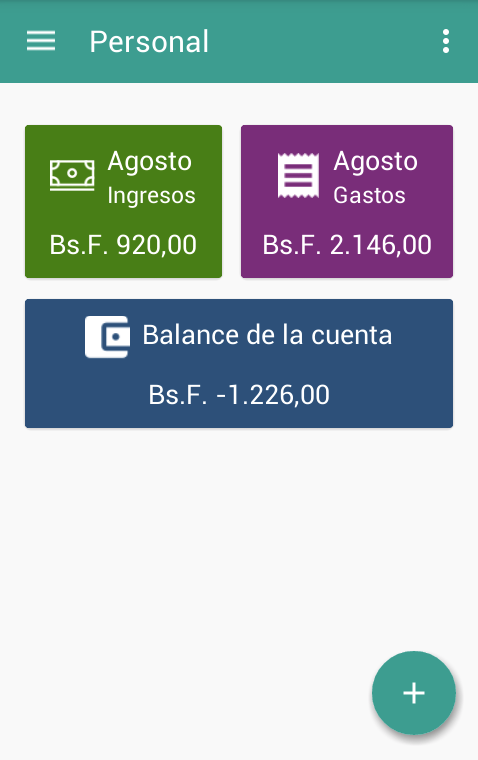
\includegraphics[scale=0.4,type=png,ext=.png,read=.png]{imagenes/dashboard}
  \captionsetup{justification=centering}
  \captionof{figure}{Interfaz principal de la\\ aplicación}
  \label{fig:interfazDashboard}
\end{minipage}%
\begin{minipage}{.5\textwidth}
\centering
  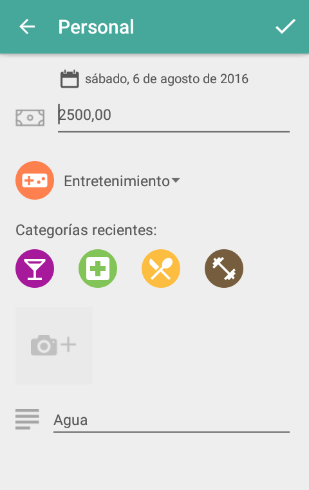
\includegraphics[scale=0.4,type=png,ext=.png,read=.png]{imagenes/create_entry}
  \captionsetup{justification=centering}
  \captionof{figure}{Interfaz para crear o editar gastos o ingresos}
  \label{fig:interfazCrearEntry}
\end{minipage}
\end{figure}

Se implementó una vista para crear y editar gastos (ver figura~\ref{fig:interfazCrearEntry}). Para estos gastos, se debe guardar su monto, fecha, descripción, fotos de recibos y categoría a la que pertenecen. Posteriormente, se extendió la funcionalidad de creación de gastos para permitir también el manejo de ingresos. 

Para mostrar los gastos e ingresos guardados, se creó una vista para listarlos (ver figuras~\ref{fig:interfazListarExpenses} y~\ref{fig:interfazListarIncomes}). En las listas se muestran la descripción/categoría a la que pertenece cada entrada, su monto y su fecha. A través de cada lista, se permite ver los detalles de cada gasto/ingreso, editarlos y eliminarlos. Además, también se permite filtrar las listas por palabras claves. 

\begin{figure}[ht]
\centering
\begin{minipage}{.5\textwidth}
  \centering
  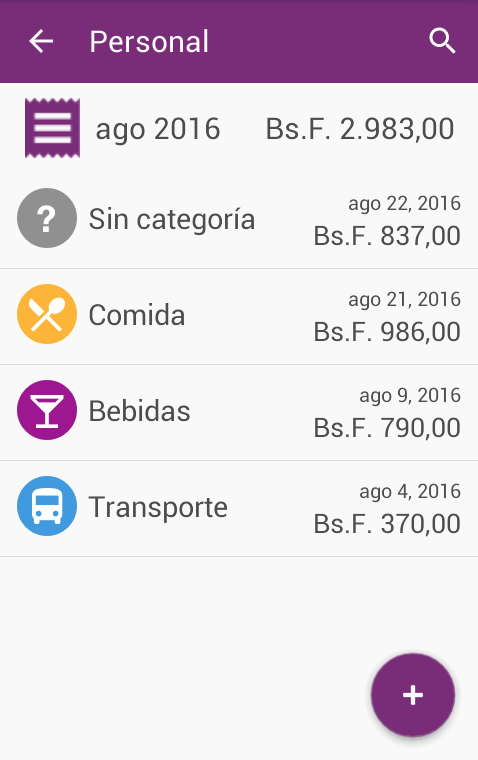
\includegraphics[scale=0.4,type=png,ext=.png,read=.png]{imagenes/expenses_list}
  \captionsetup{justification=centering}
  \captionof{figure}{Interfaz para listar gastos}
  \label{fig:interfazListarExpenses}
\end{minipage}%
\begin{minipage}{.5\textwidth}
\centering
  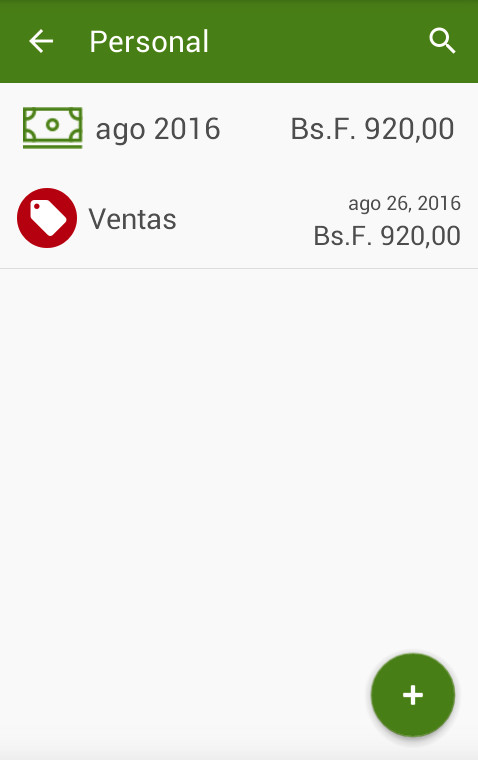
\includegraphics[scale=0.4,type=png,ext=.png,read=.png]{imagenes/incomes_list}
  \captionsetup{justification=centering}
  \captionof{figure}{Interfaz para listar ingresos}
  \label{fig:interfazListarIncomes}
\end{minipage}
\end{figure}

Para la creación de las listas, se utilizó un componente que provee Android para facilitar la tarea. Para hacer uso de él, es necesario crear una clase que actúe como intermediario entre el modelo de datos que se quiere mostrar en la interfaz de usuario, y el elemento de la interfaz que se encargará de mostrar dichos datos. Por esta razón, se utilizó el patrón de diseño \textit{Adapter} (ver capítulo~\ref{chap:Marco Teorico}) para crear la clase en cuestión.


También se crearon vistas para el manejo de categorías. Se creó una vista para la creación/edición de categorías, y otra para listarlas (ver figuras~\ref{fig:interfazListarExpenseCategories} y~\ref{fig:interfazListarIncomeCategories}). Estas categorías pueden ser de dos tipos, categorías de gastos o categorías de ingresos.

\begin{figure}[ht]
\centering
\begin{minipage}{.5\textwidth}
  \centering
  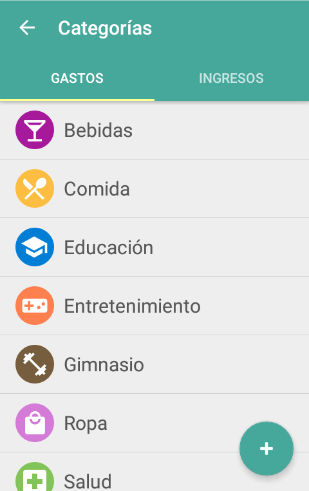
\includegraphics[scale=0.4,type=png,ext=.png,read=.png]{imagenes/expense_categories}
  \captionsetup{justification=centering}
  \captionof{figure}{Interfaz para listar categorías\\ de gastos}
  \label{fig:interfazListarExpenseCategories}
\end{minipage}%
\begin{minipage}{.5\textwidth}
\centering
  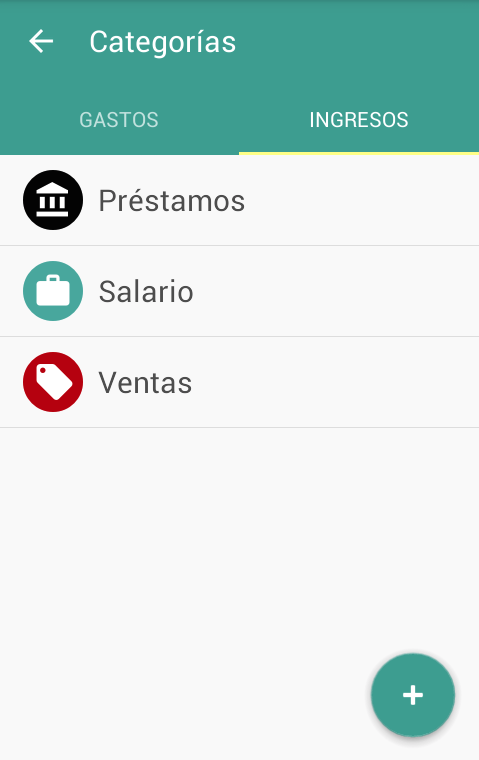
\includegraphics[scale=0.4,type=png,ext=.png,read=.png]{imagenes/income_categories}
  \captionsetup{justification=centering}
  \captionof{figure}{Interfaz para listar categorías\\ de ingresos}
  \label{fig:interfazListarIncomeCategories}
\end{minipage}
\end{figure}

Posteriormente, se implementaron funcionalidades que permiten el manejo de cuentas de ingresos/gastos. Por esta razón, también se creó una funcionalidad para agregar nuevas cuentas, y poder crear nuevos gastos e ingresos dentro de dichas cuentas. Estas cuentas pueden ser de dos tipos: activas o archivadas; la navegación entre cuentas se hace únicamente para las cuentas activas. 

Además, se creó una vista para listar las cuentas creadas y guardadas en el dispositivo (ver figuras~\ref{fig:interfazListarActiveAccounts} y~\ref{fig:interfazListarArchivedAccounts}). A partir de esta vista, se puede editar, eliminar o cambiar el estado de las cuentas (activa o archivada).


\begin{figure}[ht]
\centering
\begin{minipage}{.5\textwidth}
  \centering
  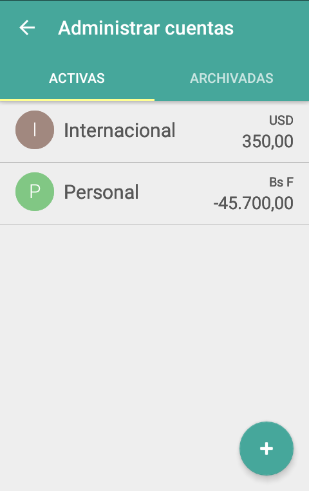
\includegraphics[scale=0.4,type=png,ext=.png,read=.png]{imagenes/active_accounts}
  \captionsetup{justification=centering}
  \captionof{figure}{Interfaz para listar cuentas\\ activas}
  \label{fig:interfazListarActiveAccounts}
\end{minipage}%
\begin{minipage}{.5\textwidth}
\centering
  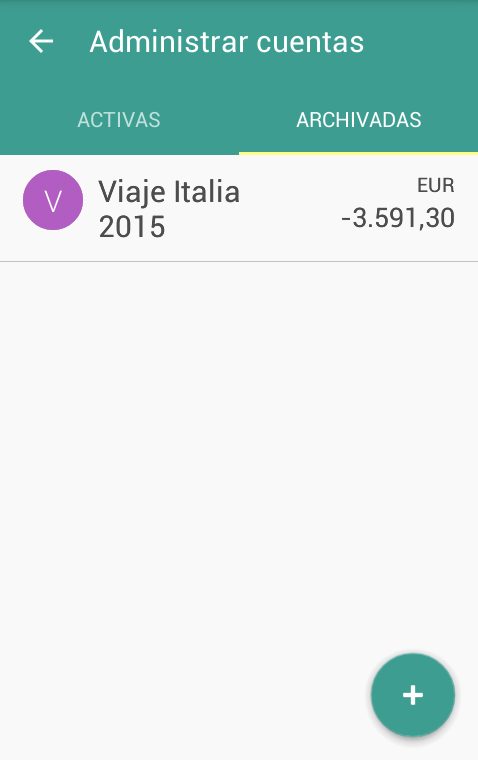
\includegraphics[scale=0.4,type=png,ext=.png,read=.png]{imagenes/archived_accounts}
  \captionsetup{justification=centering}
  \captionof{figure}{Interfaz para listar cuentas archivadas}
  \label{fig:interfazListarArchivedAccounts}
\end{minipage}
\end{figure}

\begin{figure}[ht]
\centering
\begin{minipage}{.5\textwidth}
  \centering
  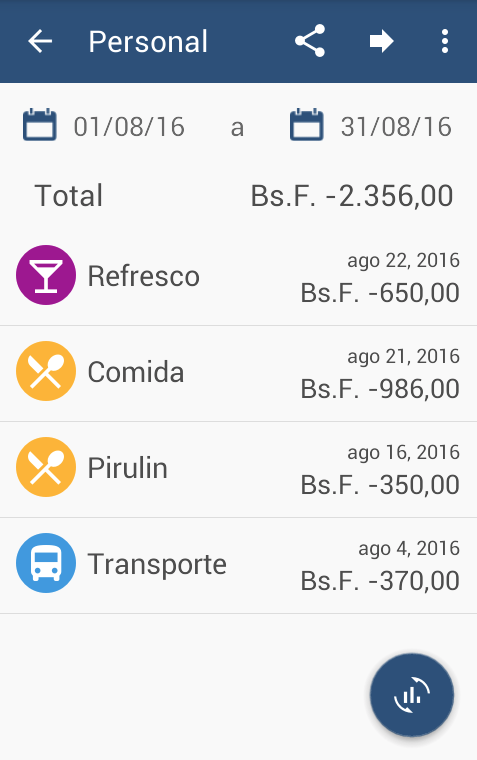
\includegraphics[scale=0.4,type=png,ext=.png,read=.png]{imagenes/balance_report}
  \captionsetup{justification=centering}
  \captionof{figure}{Interfaz para mostrar reporte\\ de balance general}
  \label{fig:interfazBalanceReport}
\end{minipage}%
\begin{minipage}{.5\textwidth}
\centering
  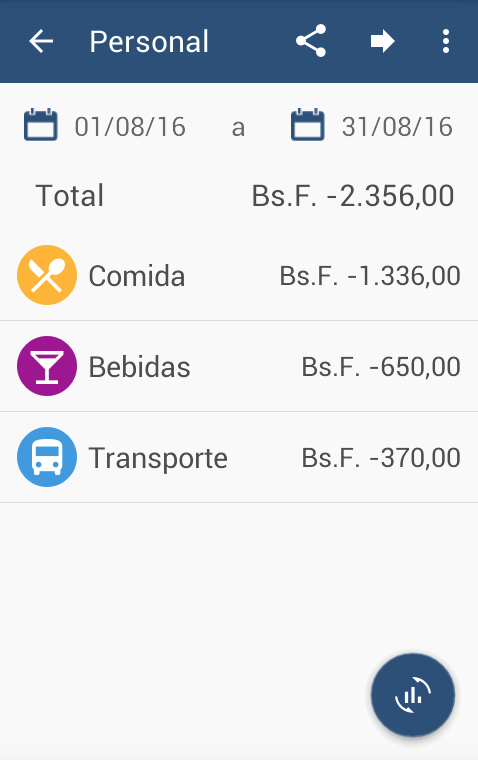
\includegraphics[scale=0.4,type=png,ext=.png,read=.png]{imagenes/categories_report}
  \captionsetup{justification=centering}
  \captionof{figure}{Interfaz para mostrar reporte\\ por categorías}
  \label{fig:interfazCategoriesReport}
\end{minipage}
\end{figure}

Además, también se crearon dos vistas para reportes de gastos: una para reportes de balance general, y otra para reporte de gastos e ingresos agrupados por categorías (ver figuras~\ref{fig:interfazBalanceReport} y~\ref{fig:interfazCategoriesReport}).

La vista de reporte de balance general muestra una lista de gastos e ingresos filtrados por fecha. La vista de reporte por categorías muestra una lista de categorías con la suma total de los gastos e ingresos de dichas categorías, filtradas por fecha.

Como se explicó en la sección anterior, es necesario guardar toda esta información en la base de datos local de cada dispositivo. Para ello, se utilizó la librería SQLite.

Para mantener la lógica separada de la interfaz gráfica, se utilizó el patrón de arquitectura MVP o Modelo Vista Presentador, descrito en el capítulo~\ref{chap:Marco Teorico}. De esta manera, toda acción en la vista que requiera realizar operaciones sobre la base de datos, se implementa por medio de una capa intermedia, conocida como presentador. Dado que el presentador es el que se comunica con el modelo para modificarlo, puede existir la necesidad de realizar estas operaciones en un hilo diferente al principal (que se encarga de actualizar la vista). Por esta razón, para la creación de las clases que actúan como presentadores, se utilizó el patrón de diseño \textit{Singleton} (ver capítulo~\ref{chap:Marco Teorico}). Con esto, se asegura la existencia de una sola instancia de cada presentador. 

Se implementó el modelo descrito en la figura~\ref{fig:diagramaClasesMovil}. Se creó la base de datos con cada una de sus tablas, así como las clases (POJO's) que permitieron dar un nivel de abstracción mayor para el mapeo con la base de datos.

También se crearon las vistas necesarias, lo que incluyó tanto las interfaces gráficas como la lógica necesaria para manejar las acciones del usuario (actividades). Para cada vista, se creó una clase que actúa como la capa de presentador, que es invocado por la vista para realizar acciones sobre el modelo. La vista se encarga de la creación de los objetos correspondientes al modelo, para luego pedir alguna acción al presentador sobre dichos objetos. El presentador tiene la función de invocar al modelo para realizar los cambios necesarios en la base de datos. Para mayor detalle de la interacción entre la vista, el modelo y el presentador, ver figuras~\ref{fig:secuenciaCrearEntry} y~\ref{fig:secuenciaGenerarReporte} del apéndice~\ref{chap:Artefactos complementarios}.

Dada la naturaleza iterativa del marco de trabajo utilizado, muchas de las funcionalidades implementadas fueron hechas a lo largo de varias iteraciones (\textit{sprints}). Por esta razón, las vistas, presentadores, así como el modelo, fueron creados y actualizados progresivamente en cada iteración.

Por otra parte, se creó un servidor al que se puede enviar información desde la aplicación móvil. 
Para esto fue necesario implementar el modelo de datos mostrado en la figura~\ref{fig:diagramaClasesServidor}. La herramienta utilizada para el desarrollo web crea por defecto una base de datos con tres tablas: \textit{User}, \textit{Role} y \textit{UserRole}. Esta base de datos se pudo adaptar al modelo de datos diseñado para el servidor, por lo que únicamente fue necesario crear la tabla \textit{Report}.

Todos los servicios web se crearon basándose en el estilo arquitectónico REST (ver capítulo~\ref{chap:Marco Teorico}). 

Para permitir el acceso a la aplicación móvil, se creó un servicio web que permita hacer la autenticación del usuario. La aplicación envía al servidor un JSON con los datos del usuario (nombre de usuario y contraseña) por medio de una petición HTTP POST.

Se creó un servicio web que recibe un archivo PDF cuyo contenido es un reporte de gastos e ingresos. Además del archivo, recibe un JSON que contiene la suma de gastos por cada categoría de interés para la empresa, el mes y el año del reporte. Estos datos se enviaron por medio de una petición HTTP POST con Content-Type Multipart, cuyo cuerpo está compuesto por un archivo y un JSON. Para la conversión de objetos de Java a JSON, y viceversa, se utilizó la librería GSON tanto en el servidor como en la aplicación móvil. Para persistir esta información, se utilizó Hibernate y MySQL como manejador de base de datos.

También se desarrolló una aplicación web que permite aprobar o rechazar los reportes enviados al servidor, así como ver los reportes recibidos y ya revisados (ver figuras~\ref{fig:interfazListarReportesPendientes} y~\ref{fig:interfazListarReportesRevisados}). 

\begin{figure}[ht]
  \centering
  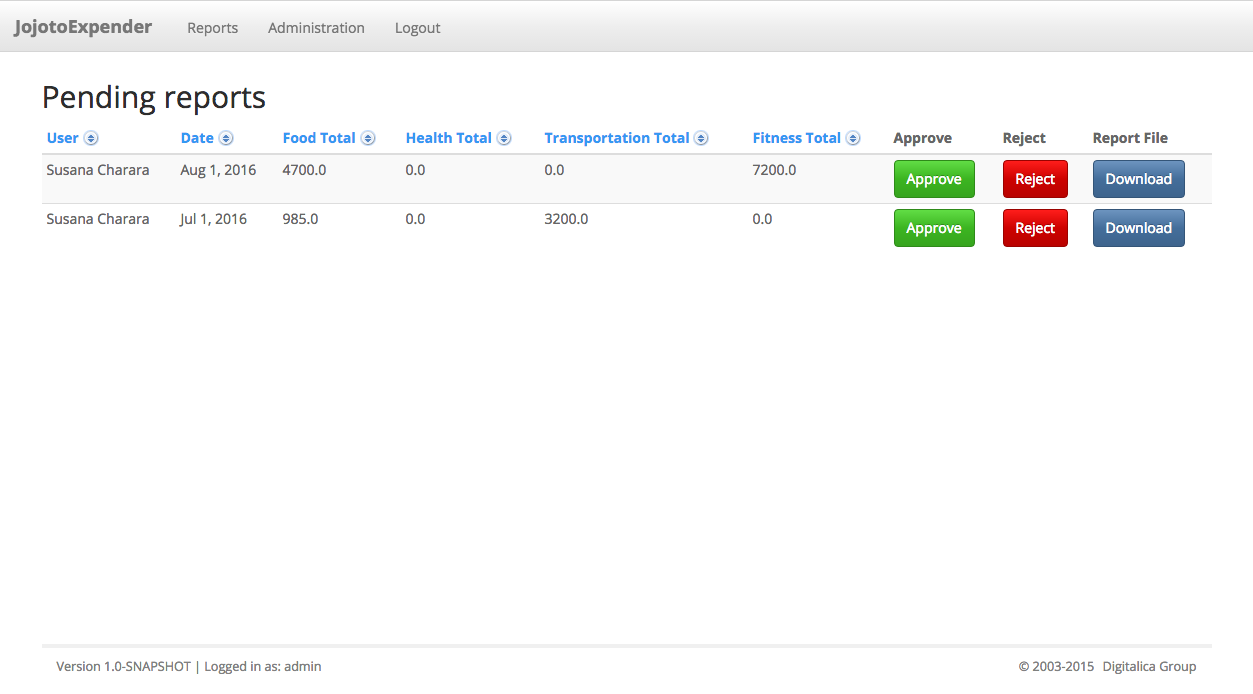
\includegraphics[scale=0.38,type=png,ext=.png,read=.png]{imagenes/pending_reports}
  \captionsetup{justification=centering}
  \caption{Interfaz para listar reportes pendientes de revisión}
  \label{fig:interfazListarReportesPendientes}
\end{figure}

\begin{figure}[ht]
  \centering
  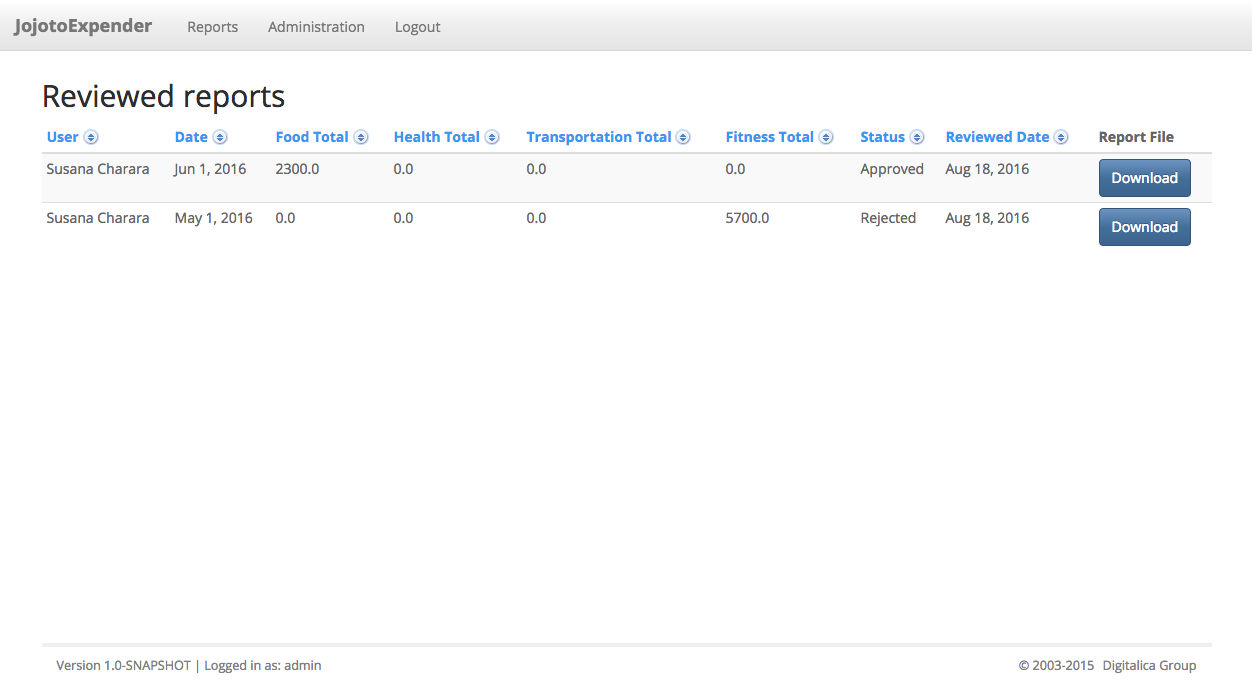
\includegraphics[scale=0.38,type=png,ext=.png,read=.png]{imagenes/reviewed_reports}
  \captionsetup{justification=centering}
  \caption{Interfaz para listar reportes aprobados/rechazados}
  \label{fig:interfazListarReportesRevisados}
\end{figure}


Se creó una funcionalidad para notificar a los supervisores vía correo electrónico cuando un nuevo reporte es recibido en el servidor; este correo electrónico incluye el archivo PDF del reporte. Asimismo, cuando un supervisor toma la decisión de aprobar o rechazar un reporte, se notifica por correo electrónico al usuario que envió dicho reporte.

Además de esto, la herramienta utilizada para el desarrollo del servidor trae consigo algunas funcionalidades por defecto (incluyendo las vistas web necesarias) que permiten iniciar sesión, agregar un usuario, editar un usuario y eliminar un usuario. 

El desarrollo del componente servidor se realizó con el IDE Eclipse. Se utilizó el \textit{framework} AppFuse, que unifica a su vez otros \textit{frameworks} que facilitan el desarrollo web. En este caso, se trabajó en conjunto con Spring y Tapestry.

Se utilizó Spring para la implementación de los servicios web que permiten recibir datos desde la aplicación móvil. Estos servicios se implementaron utilizando el patrón Fachada o \textit{Facade} (ver capítulo~\ref{chap:Marco Teorico}); se implementó una clase \textit{Manager} para exponer los servicios web, que actúa como una fachada para los DAO. Además, AppFuse también cuenta con el \textit{framework} Hibernate para la persistencia de los datos, utilizando como manejador de base de datos MySQL.

Para crear la aplicación web, se utilizó Tapestry. Con Jetty se proveen los servicios, mediante el protocolo HTTP, que permiten la comunicación con la aplicación web y la aplicación  móvil.

Por otra parte, a través de la librería Retrofit, la aplicación móvil se comunica con el servidor web utilizando el protocolo HTTP. La comunicación con la base de datos del dispositivo y con los servicios web se realiza en la capa del presentador. Por su parte, en la vista se maneja toda la interfaz gráfica a través de la cual el usuario interactúa con la aplicación móvil, y toda la lógica necesaria para la comunicación con la capa de modelo y el presentador.

El proyecto se desarrolló bajo el marco de trabajo de \textit{Scrum}, descrito en el capítulo~\ref{chap:Marco Metodologico}. Durante la ejecución de las iteraciones, se implementaron las funcionalidades planificadas. Para cada una de ellas, se realizaron las pruebas necesarias para validarlas (para más información, consultar el plan de pruebas en el apéndice~\ref{chap:Plan de pruebas}). 

A continuación se presentarán las iteraciones (\textit{sprints}), durante las cuales se desarrollaron las funcionalidades descritas en los párrafos anteriores. Para cada iteración, se mencionarán sus objetivos y resultados, con una breve descripción de las actividades realizadas.

\subsection{Iteración 1}

\subsubsection{Objetivos}
	\begin{itemize}
  \item Implementar el modelo de datos de la aplicación móvil.
	\item Crear la vista principal de la aplicación.
	\item Permitir la creación de un nuevo gasto.
	\end{itemize}

\subsubsection{Resultados}
\begin{itemize}
\item Se implementó el modelo de datos de la aplicación móvil, que permite persistir toda la información necesaria para la misma. Se creó la base de datos con la librería SQLite, las tablas necesarias para cumplir con el modelo de datos de la figura~\ref{fig:diagramaClasesMovil}, así como los POJO's correspondientes.
\item Se creó la vista principal de la aplicación, a través de la cual el usuario puede consultar de la base de datos el total de ingresos, gastos y balance general. Se creó una interfaz de usuario con tres elementos que muestran dichos montos (figura~\ref{fig:interfazDashboard}).
\item Se creó una vista para permitir la creación de un nuevo gasto con su fecha, monto y descripción. Un gasto representa un registro dentro de la tabla correspondiente a la clase \textit{Expense} (figura~\ref{fig:diagramaClasesMovil}). Se creó una interfaz de usuario que incluye los campos necesarios para ingresar la fecha, el monto y la descripción del gasto. Además, se creó una consulta para agregar a la base de datos un nuevo gasto.
\end{itemize}

%\subsubsection{Actividades}
%En la primera parte de la iteración se implementó el modelo de datos del dispositivo móvil, lo que implicó la creación de la base de datos con sus tablas, así como los POJO's correspondientes.
%
%Se creó la vista principal de la aplicación móvil, que implicó la creación de una interfaz de usuario con tres elementos que muestran el total de ingresos, el total de gastos y el balance general (figura ~\ref{fig:interfazDashboard}). Para esto, fue necesario crear consultas a la base de datos que permitieran obtener el total de ingresos/gastos de una cuenta.  También se realizó una consulta que permite obtener el balance total de una cuenta.
%
%Por otro lado se implementó una vista que permite crear un nuevo gasto, con su fecha, monto y descripción. Se creó una interfaz de usuario que incluye los campos necesarios para ingresar la fecha, el monto y la descripción del gasto. Además, se creó una consulta para agregar a la base de datos un nuevo gasto.

\subsection{Iteración 2}

\subsubsection{Objetivos}
\begin{itemize}
\item Mostrar la lista de categorías.
\item Permitir la creación de un nuevo ingreso.
\item Permitir guardar fotos de un ingreso/gasto.
\item Asociar un ingreso/gasto a una categoría.
\end{itemize}

\subsubsection{Resultados}
\begin{itemize}
\item Se creó una vista para mostrar la lista de categorías a las que puede pertenecer un gasto. Una categoría es un registro dentro de la tabla \textit{Category} (figura~\ref{fig:diagramaClasesMovil}); en este sentido, la vista permite al usuario consultar de la base de datos del dispositivo los registros correspondientes a la tabla \textit{Category}. Estas categorías pueden ser de dos tipos: ingresos o gastos. Por esta razón, se creó una interfaz que muestra dos listas de categorías, una para cada tipo (figuras~\ref{fig:interfazListarExpenseCategories} y~\ref{fig:interfazListarExpenseCategories}). Para cada categoría, se muestra su nombre y su ícono. Además de esto, se creó una funcionalidad para guardar en la base de datos una lista de categorías por defecto. Esto implicó la creación de una consulta para agregar a la base de datos una nueva categoría, con su nombre y su ícono.
\item Se adaptó la vista creada en la iteración 2, a través de la cual se puede crear un gasto, de manera que permitiera la creación de un ingreso. Un ingreso representa un registro dentro de la tabla correspondiente a la clase \textit{Income} (figura~\ref{fig:diagramaClasesMovil}). Como se observó en la figura~\ref{fig:diagramaClasesMovil}, un ingreso y un gasto guardan la misma información; por esta razón, no fue necesario cambiar la interfaz ya creada, sino que se cambió la lógica detrás de ella para identificar si se está usando para crear un ingreso o un gasto.
\item Se agregó una funcionalidad para capturar y guardar fotos relacionadas a un ingreso/ gasto; esto permite que, por ejemplo, el usuario pueda guardar en el dispositivo móvil fotos de los recibos de los gastos. Para esto se creó un método que permite abrir alguna aplicación instalada en el dispositivo, a través de la cual se puedan capturar y guardar fotos. Una vez guardadas, se inserta dentro de la tabla \textit{Photo} la ruta donde están ubicadas las fotos dentro del dispositivo. Se adaptó la vista para la creación de un ingreso/gasto para mostrar las miniaturas de las fotos tomadas.% Se puso un límite por parte de la empresa para que el máximo de fotos que se puedan guardar por ingreso/gasto sean 3.
\item Se agregó una funcionalidad para poder asociar un ingreso/gasto a una categoría existente, lo que permite al usuario especificar a qué rubro pertenece el gasto o ingreso, según sea el caso. Con esta funcionalidad, el usuario puede insertar, dentro de las tablas correspondiente a las clases \textit{Income} y \textit{Expense}, la categoría a la que pertenece dicho ingreso o gasto. Se modificó la vista para la creación de un ingreso/gasto, pues se tuvo que agregar un nuevo elemento a la interfaz, a través del cual se muestran las categorías guardadas en la base de datos, y de las cuales se puede seleccionar una para asociarla al ingreso/gasto.

Se tenía como requerimiento guardar las cuatro categorías que se utilizaron más recientemente. Para esto, se tuvo que crear los métodos necesarios para persistir en el dispositivo móvil las categorías más recientes. Dado que esta información no tiene una estructura compleja, se decidió utilizar un objeto que provee la plataforma de Android, llamado \textit{SharedPreferences}, que permite guardar un conjunto de pares clave-valor. Este objeto permite persistir las categorías más recientes, aún cuando se cierre la aplicación.

\end{itemize}

%\subsubsection{Actividades}
%
%En esta iteración se creó una vista para mostrar las categorías presentes en la base de datos del dispositivo. Como se mencionó anteriormente, las categorías pueden ser de dos tipos: ingresos o gastos. Por esta razón, se creó una interfaz que permita mostrar dos listas de categorías, una para cada tipo. Para cada categoría, se muestra su nombre y su ícono.
%
%Además de esto, se creó una funcionalidad para guardar en la base de datos una lista de categorías por defecto. Esto implicó la creación de una consulta que permita agregar a la base de datos una nueva categoría, con su nombre y su ícono.
%
%También se adaptó la vista existente para la creación de un gasto, de manera que se pueda reutilizar esta vista para la creación de un ingreso. Como se observó en la figura ~\ref{fig:diagramaClasesMovil}, un ingreso y un gasto guardan la misma información. Por esta razón, no fue necesario cambiar la interfaz ya creada, sino que se cambió la lógica detrás de ella para identificar si se está usando para crear un ingreso o un gasto.
%
%Por otra parte, se implementó la funcionalidad para tomar y guardar fotos asociadas a un ingreso/gasto. Para esto se creó un método que permita abrir alguna aplicación para el manejo de la cámara, que esté instalada en el dispositivo. Con esta aplicación se capturan las fotos. 
%
%Luego, se tuvo que adaptar la vista para la creación de un ingreso/gasto para mostrar las miniaturas de las fotos tomadas. Se puso un límite por parte de la empresa para que el máximo de fotos que se puedan guardar por ingreso/gasto sean 3.
%
%Por último, se modificó la vista para la creación de un ingreso/gasto, de manera que se permitiera asociar una categoría. Esto implicó agregar un nuevo elemento a la interfaz, a través del cual se muestran y se pueden seleccionar las categorías guardadas en la base de datos. 
%
%Se tenía como requerimiento guardar las cuatro categorías que se utilizaron más recientemente. Para esto, se tuvo que crear los métodos necesarios para persistir en el dispositivo móvil las categorías más recientes. Dado que esta información no tiene una estructura compleja, se decidió utilizar un objeto que provee la plataforma de Android, llamado \textit{SharedPreferences}, que permite guardar un conjunto de pares clave-valor. En este caso, se guardó una lista con las categorías más recientes. Este objeto permitió persistir las categorías más recientes, aún cuando se cierre la aplicación.

\subsection{Iteración 3}
\subsubsection{Objetivos}
\begin{itemize}
\item Mostrar la lista de ingresos/gastos del mes actual.
\item Mostrar los detalles de los ingresos/gastos existentes.
\item Permitir editar y borrar un ingreso/gasto existente.
\item Implementar una calculadora para guardar el monto de un ingreso/gasto.
\end{itemize}

\subsubsection{Resultados}
\begin{itemize}
\item Se implementó una funcionalidad para navegar a la lista de ingresos o de gastos del mes, desde la vista principal de la aplicación. Esta funcionalidad permite al usuario consultar los registros de las tablas que corresponden a las clases \textit{Income} y \textit{Expense}, según sea el caso. Dado que se guarda la misma información para ingresos y gastos, se creó una vista general donde se puede mostrar la lista deseada. Se creó una interfaz que permite mostrar una lista de ingresos/gastos con su descripción (o categoría, en caso de que no tenga descripción), su fecha y su monto. Esta vista se reutilizó para mostrar tanto los ingresos como los gastos, según sea necesario (ver figuras~\ref{fig:interfazListarExpenses} y \ref{fig:interfazListarIncomes}).
\item Se agregó una funcionalidad para ver los detalles de un ingreso/gasto ya existente, y poder editarlo. Con esta funcionalidad, el usuario puede consultar la información relacionada con los ingresos/gastos guardados en la base de datos, así como actualizarla. Para esto no fue necesario crear una interfaz nueva, sino que se reutilizó la que se tenía para la creación de un nuevo ingreso/gasto. Se adaptó la vista correspondiente, de manera que se pueda detectar si se quiere crear un nuevo ingreso/gasto, o si por el contrario se quiere editar uno ya existente. En caso de que exista, se llenan automáticamente los campos de la fecha, monto, categoría, descripción y fotos.
\item Se agregó una funcionalidad para eliminar ingresos/gastos. Esto permite al usuario eliminar ingresos y gastos de la base de datos del dispositivo, a través de la vista donde se listan los mismos. Además, se tuvo que realizar cambios a la lógica detrás de la interfaz creada, de manera que se permitiera seleccionar filas de la lista (en este caso las filas corresponden a ingresos o gastos que se deseen eliminar, ver figura~\ref{fig:interfazEliminarGastos}). 
\item Se creó una interfaz para usar una calculadora que permita ingresar el monto de un ingreso/gasto. Se modificó la vista de creación de un ingreso/gasto para incluir la nueva funcionalidad. 

Para este último requerimiento fue necesario crear un teclado virtual personalizado, pues el teclado numérico del dispositivo no incluye los operadores matemáticos básicos. Para esto se creó una interfaz en la que se especificó la disposición de las teclas de la calculadora (ver figura~\ref{fig:interfazCalculadora}). También se tuvo que manejar el uso de las teclas: dentro de la vista, se creó la lógica para detectar qué tecla fue presionada y realizar una acción en base a esto. Para realizar los cálculos, se utilizó una librería que evalúa fórmulas dada una cadena de caracteres. En este caso, la cadena de caracteres representa las teclas presionadas.

Para la calculadora, se tiene que mostrar el símbolo decimal de acuerdo con el país para el cual está configurado el teléfono, ya que en algunos países se usa la coma (,) como separador y en otros el punto (.). Por esta razón, se debe obtener el país de configuración del teléfono y, en base a eso, decidir qué símbolo decimal mostrar.

\end{itemize}
%
%\subsubsection{Actividades}
%
%En la primera iteración, se mostraba en la vista principal el total de ingresos y de gastos de una cuenta, desde su creación. En esta iteración se quería mostrar únicamente el total del mes actual. Por esta razón, se tuvo que modificar la consulta a la base de datos para obtener el total de ingresos/gastos dado un rango de fecha.
%
%Se implementó una funcionalidad para navegar a la lista de ingresos o de gastos del mes desde la vista principal de la aplicación. Dado que se guarda la misma información para ingresos y gastos, se creó una vista general donde se pueda mostrar una lista de ingresos/gastos. Se creó una interfaz que permite mostrar una lista de ingresos/gastos con su descripción (o categoría, en caso de que no tenga descripción), su fecha y su monto. Esta vista se reutilizó para mostrar tanto los ingresos como los gastos, según sea el caso.
%
%Por otra parte, se creó la funcionalidad para eliminar ingresos/gastos existentes desde la vista mencionada en el párrafo anterior. Se creó una consulta que permitiera eliminar de la base de datos un ingreso/gasto. Además, se tuvo que realizar cambios a la lógica detrás de la interfaz creada, de manera que se permitiera seleccionar filas de la lista (en este caso las filas corresponden a ingresos o gastos que se deseen eliminar, ver apéndice~\ref{fig:interfazEliminarGastos}). 
%
%También se creó la funcionalidad para editar un ingreso/gasto existente. Para esto no fue necesario crear una interfaz nueva, sino que se reutilizó la que se tenía para la creación de un nuevo ingreso/gasto. Se adaptó la vista correspondiente, de manera que se pueda detectar si se quiere crear un nuevo ingreso/gasto, o si por el contrario se quiere editar uno ya existente. En caso de que exista, se llenan automáticamente los campos de la fecha, monto. categoría, descripción y fotos con los datos existentes del ingreso/gasto que se quiere editar.
%
%Por último, se tenía como requerimiento mostrar una calculadora para ingresar el monto de un ingreso/gasto, en lugar de un teclado numérico común. Por esta razón, se tuvo que modificar la vista de creación de un ingreso/gasto para incluir la nueva funcionalidad. 
%
%Para este último requerimiento fue necesario crear un teclado virtual personalizado, pues el teclado numérico del dispositivo no incluye los operadores matemáticos básicos. Para esto se creó una interfaz en la que se especificó la disposición de las teclas de la calculadora, que las teclas presentes en una calculadora básica (ver apéndice~\ref{fig:interfazCalculadora}). También se tuvo que manejar el uso de las teclas: dentro de la vista, se tuvo que crear la lógica para detectar qué tecla fue presionada y realizar una acción en base a esta. Para realizar los cálculos, se utilizó una librería para evaluar fórmulas dada una cadena de caracteres. En este caso, la cadena de caracteres representa las teclas presionadas.
%
%Para la calculadora, se tenía que mostrar el símbolo decimal de acuerdo con el país para el cual está configurado el teléfono, ya que en algunos países se usa la coma (,) como separador y en otros el punto (.). Por esta razón, se tuvo que obtener el país de configuración del teléfono y, en base a eso, decidir qué símbolo decimal mostrar.

\subsection{Iteración 4}
\subsubsection{Objetivos}
\begin{itemize}
\item Permitir el manejo de nuevas cuentas.
\end{itemize}

\subsubsection{Resultados}
\begin{itemize}

\item Se creó una vista para crear una nueva cuenta. Una cuenta representa un registro dentro de la tabla \textit{Account}(figura~\ref{fig:diagramaClasesMovil}). Así, esta vista permite insertar en la base de datos un registro dentro de la tabla \textit{Account}. Se creó una interfaz de usuario, con campos para ingresar el nombre y la moneda en la que estará la nueva cuenta (ver figura~\ref{fig:interfazCrearCuenta}). También fue necesario crear una consulta para agregar a la base de datos una cuenta.
\item Se implementó una funcionalidad para listar las cuentas del usuario. Esta vista le permite al usuario consultar de la base de datos del dispositivo todos los registros correspondientes a la tabla \textit{Account}. Se creó una interfaz que contiene una lista, y las filas corresponden a cuentas. Para cada cuenta, se muestra su nombre, la moneda y el balance general de la misma. Fue necesario crear una consulta a la base de datos para obtener todas las cuentas guardadas en el dispositivo.
\item Se implementó una funcionalidad para navegar entre cuentas, lo que permite cambiar la cuenta que se está mostrando actualmente en el dispositivo. Se creó una barra lateral (\textit{sidebar}) en la vista principal de la aplicación (ver figura~\ref{fig:interfazCambiarCuenta}) en la que se muestra la lista de cuentas activas en el dispositivo. Para mostrar dicha lista, se realiza una consulta a la base de datos para obtener todos los registros de la tabla \textit{Account} cuyo \textit{status} sea \textit{activa}. De la lista de cuentas que se muestra, se puede seleccionar alguna para que sea la que se esté mostrando actualmente en el dispositivo. La cuenta seleccionada se persistió mediante un \textit{SharedPreferences}, de manera que esta información queda guardada en caso de que se cierre la aplicación.
\item Se implementó una funcionalidad para editar el nombre de una cuenta existente. Con esto, se permite al usuario modificar el campo \textit{name} de un registro de la tabla \textit{Account}(figura~\ref{fig:diagramaClasesMovil}). Fue necesario adaptar la vista existente para la creación de una cuenta, de manera que se permita editar una ya existente. Dentro de la vista, se creó la lógica necesaria para detectar si se está creando una nueva cuenta o si se está editando. En caso de que se esté editando, se llenan los campos del nombre y la moneda. Para persistir los cambios realizados, se creó una consulta a la base de datos que permite actualizar la información de una cuenta. 
\item Se implementó una funcionalidad para eliminar cuentas existentes. Esta funcionalidad permite al usuario eliminar registros de la tabla \textit{Account}. Se modificó la vista de la lista de cuentas de manera que se puedan seleccionar las cuentas que se desean eliminar (ver figura~\ref{fig:interfazEliminarCuentas}). También se creó una consulta a la base de datos para eliminar cuentas de la misma.
\item Se implementó una funcionalidad para cambiar el estado de una cuenta: activa o archivada; esto permite que el usuario pueda modificar el campo \textit{status} de un registro de la tabla \textit{Account}. Fue necesario la creación de una consulta que permita cambiar el estado de una cuenta en la base de datos. La lista de cuentas se muestra según su estado, es decir, se muestra una lista para la lista de cuentas activas y una para las cuentas archivadas. 
\item Se implementó una funcionalidad que permite al usuario consultar de la base de datos todos los registros correspondientes tanto a ingresos como a gastos. Hasta ahora, desde la vista principal de la aplicación se podía navegar a la lista de ingresos y la lista de gastos del mes actual, por separado. Se agregó una nueva funcionalidad para navegar a una lista que contenga todos los ingresos y gastos de una cuenta, y que no esté limitada al mes actual. Esto no implicó la modificación de la interfaz, sino de la lógica a través de la cual se puede saber qué lista se está mostrando. Se creó una consulta a la base de datos para obtener una lista con todos los ingresos y gastos de una cuenta, sin estar limitado a un rango de fechas.
\end{itemize}
%
%\subsubsection{Actividades}
%En la ejecución de las iteraciones anteriores, no se manejaban cuentas. Para esta iteración, se decidió agregar una funcionalidad para poder manejar nuevas cuentas. 
%
%Para esto, se creó una vista que permite agregar una nueva cuenta. Se creó una interfaz de usuario, con campos para ingresar el nombre y la moneda en la que estará la nueva cuenta (ver apéndice~\ref{fig:interfazCrearCuenta}). También fue necesario crear una consulta para agregar a la base de datos una cuenta.
%
%Se creó una vista para mostrar la lista de cuentas guardadas. Esto incluyó la creación de una interfaz que contiene una lista, y las filas corresponden a cuentas. Para cada cuenta, se muestra su nombre, la moneda y el balance general de la misma. Fue necesario crear una consulta a la base de datos para obtener todas las cuentas guardadas en el dispositivo.
%
%Se implementó una funcionalidad para cambiar el estado de una cuenta: activa o archivada. Esto implicó modificar la vista de la lista de cuentas de manera que se puedan seleccionar las cuentas a las que se les quiere cambiar el estado (ver apéndice~\ref{fig:interfazEliminarCuentas}). Fue necesario la creación de una consulta que permita cambiar el estado de una cuenta en la base de datos. La lista de cuentas se muestra según su estado, es decir, se muestra una lista para la lista de cuentas activas y una para las cuentas archivadas. 
%
%Además, se implementaron funcionalidades para editar el nombre de una cuenta y eliminar cuentas ya existentes. Fue necesario adaptar la vista existente para la creación de una cuenta, de manera que se permita editar una ya existente. Dentro de la vista, se creó la lógica necesaria para detectar si se está creando una nueva cuenta o si se está editando. En caso de que se esté editando, se llenan los campos del nombre y la moneda.
%
%Se crearon consultas a la base de datos que permitieran la modificación y eliminación de cuentas.
%
%También se creó una funcionalidad para cambiar la cuenta que se está mostrando actualmente en el dispositivo. Se creó una barra lateral (\textit{sidebar}) en la vista principal de la aplicación (ver apéndice~\ref{fig:interfazCambiarCuenta}). En ella, se muestra la lista de cuentas activas en el dispositivo, de las cuales se puede seleccionar alguna para que sea la que se esté mostrando actualmente en el dispositivo. Se persistió mediante un \textit{SharedPreferences} la cuenta seleccionada, de manera que esta información quede guardada en caso de que se cierre la aplicación.
%
%Por último, se adapto la vista existente para mostrar la lista de ingresos/gastos, de manera que se pueda mostrar todos los ingresos/gastos (en una misma lista) asociados a la cuenta que se muestra actualmente. Hasta ahora, desde la vista principal de la aplicación se podía navegar a la lista de ingresos y la lista de gastos del mes actual, por separado. Se agregó una nueva funcionalidad para navegar a una lista que contenga todos los ingresos y gastos de una cuenta, y que no esté limitada al mes actual. Esto no implicó la modificación de la interfaz, sino de la lógica a través de la cual se puede saber qué lista se está mostrando. Se creó una consulta a la base de datos para obtener una lista con todos los ingresos y gastos de una cuenta, sin estar limitado a un rango de fechas.

\subsection{Iteración 5}
\subsubsection{Objetivos}
\begin{itemize}
\item Permitir el manejo de las fotos de un ingreso/gasto.
\item Permitir el manejo de las categorías.
\end{itemize}

\subsubsection{Resultados}
\begin{itemize}
\item Se agregó una funcionalidad para ver las fotos de un ingreso/gasto. Esto permite al usuario hacer una consulta a la base de datos para obtener los registros de la tabla \textit{Photo} asociados a un ingreso/gasto. Se creó una vista que muestra en pantalla completa las fotos de un ingreso/gasto (esto se hace desde la vista de creación de un ingreso/gasto). Esto implicó la creación de la interfaz y la lógica que permita seleccionar una foto, abrirla y mostrarla en pantalla completa (ver figura~\ref{fig:interfazVerFoto}).
\item Se agregó una funcionalidad para borrar las fotos de un ingreso/gasto, a través de la cual el usuario puede realizar una consulta para eliminar de la base de datos registros de la tabla \textit{Photo}, así como eliminar los archivos de las fotos dentro del dispositivo. Se agregó un elemento a la interfaz mencionada en el punto anterior, a través del cual se pueden eliminar las fotos(ver figura~\ref{fig:interfazEliminarFoto}).
\item Se agregó una funcionalidad para cambiar la ubicación en el dispositivo móvil de las fotos tomadas de un ingreso/gasto. Para esto se creó una vista de configuraciones de la aplicación, a través de la cual se puede cambiar la ubicación donde se guardarán las fotos tomadas. Esto implica cambiar la ubicación de las fotos tomadas anteriormente, y que las nuevas fotos que serán tomadas se guardarán en la nueva ubicación.

Se creó una interfaz donde se muestra la ubicación actual (carpeta) de las fotos. Además, se agregaron dos opciones para cambiar la ubicación en el dispositivo en la que se guardan los archivos de las fotos: memoria interna o memoria extraíble (ver figura~\ref{fig:interfazConfiguracion}). También fue necesario crear la lógica que se encarga de cambiar a la nueva ubicación las fotos tomadas anteriormente.
\item Se agregó una vista para crear una categoría. A través de ella, se hace una consulta a la base de datos para insertar un nuevo registro dentro de la tabla \textit{Category}. Se creó una interfaz de usuario con elementos que permiten ingresar el nombre de la categoría y un ícono (ver figura~\ref{fig:interfazCrearCategoria}). Las imágenes de los íconos a los cuales se puede asociar una categoría están guardadas por defecto dentro de la aplicación. Se creó un campo a través del cual se muestran los íconos que aún no han sido utilizados, y de los cuales se debe escoger uno. La consulta para agregar una nueva categoría a la base de datos fue creada en la iteración 2, como se mencionó anteriormente.
\item Se agregó una funcionalidad para eliminar, a través de una vista, registros de la tabla \textit{Category}. Para esto, se adaptó la interfaz creada en la iteración 2, a través de la cual se muestra la lista de categorías presentes en el dispositivo (ver figura~\ref{fig:interfazEliminarCategorias}). Esta adaptación se hizo para permitir seleccionar las categorías que se desean eliminar. Se creó una consulta a la base de datos para eliminar de la misma una categoría. También fue necesario crear una consulta para verificar qué ingresos/gastos están asociados a las categorías que se quieren eliminar; a estos ingresos/gastos se les deja sin categoría, y posteriormente se eliminan las categorías deseadas de la base de datos.
\item Se agregó una funcionalidad para editar una categoría existente; con ella, se permite al usuario realizar consultas sobre la base de datos del dispositivo para actualizar registros de la tabla \textit{Category}. Se modificó la vista existente para la creación de una nueva categoría, de manera que soportara también la edición. No se modificó la interfaz gráfica sino que se creó la lógica para verificar si se trata de una nueva categoría o de una ya existente que se quiere editar. En caso de que sea una existente, se muestra la información correspondiente (nombre e ícono). Se creó una consulta a la base de datos para persistir los cambios una vez editada una categoría.
\end{itemize}

%\subsubsection{Actividades}
%La primera parte de la iteración se dedicó al manejo de las fotos. En primer lugar se creó la vista para poder ver en pantalla completa las fotos de un ingreso/gasto (esto se hace desde la vista de creación de un ingreso/gasto). Esto implicó la creación de la interfaz y la lógica que permita seleccionar una foto, abrirla y mostrarla en pantalla completa (ver apéndice~\ref{fig:interfazVerFoto}).
%
%También se implementó la funcionalidad para eliminar una foto, para lo que se tuvo que crear una consulta a la base de datos para eliminar registros de la tabla correspondiente. También se agregó un elemento a la interfaz para mostrar fotos, a través del cual se pueden eliminar (ver apéndice~\ref{fig:interfazEliminarFoto}).
%
%Por otra parte, se creo la vista de configuraciones de la aplicación, a través de la cual se puede cambiar la ubicación donde se guardarán las fotos tomadas. Esto implica cambiar la ubicación de las fotos tomadas anteriormente, y que las nuevas fotos que serán tomadas se guardarán en la nueva ubicación.
%
%Se creó una interfaz donde se muestra la ubicación actual (carpeta) de las fotos. Además, se agregaron dos opciones para cambiar la ubicación en el dispositivo en la que se guardan los archivos de las fotos: memoria interna o memoria extraíble (ver apéndice~\ref{fig:interfazConfiguracion}). También fue necesario crear la lógica que se encarga de cambiar a la nueva ubicación las fotos tomadas anteriormente.
%
%La segunda parte de la iteración se dedicó al manejo de las categorías. 
%
%Se creó la vista para agregar una nueva categoría, lo que implicó la creación de una interfaz de usuario con elementos que permiten ingresar el nombre de la categoría y un ícono (ver apéndice~\ref{fig:interfazCrearCategoria}). Las imágenes de los íconos a los cuales se puede asociar una categoría están guardadas por defecto dentro de la aplicación. Se creó un campo a través del cual se muestran los íconos que aún no han sido utilizados, y de los cuales se debe escoger uno. La consulta para agregar una nueva categoría a la base de datos fue creada en la iteración 2, como se mencionó anteriormente.
%
%Se modificó la vista existente para la creación de una nueva categoría, de manera que se soporte también la edición. Como ocurrió con las cuentas, no se modificó la interfaz gráfica sino la lógica que se encarga de verificar si se trata de una nueva categoría o de una ya existente que se quiere editar. En caso de que sea una existente, se muestra la información correspondiente (nombre e ícono). Se creó una consulta a la base de datos para persistir los cambios una vez editada una categoría.
%
%Por último, se agregó una funcionalidad para poder eliminar categorías. Para esto, se adaptó la interfaz creada en la iteración 2, a través de la cual se muestra la lista de categorías presentes en el dispositivo (ver apéndice~\ref{fig:interfazEliminarCategorias}). Esta adaptación se hizo para permitir seleccionar las categorías que se desean eliminar. Se creó una consulta a la base de datos para eliminar de la misma una categoría. También fue necesario crear una consulta para verificar qué ingresos/gastos están asociados a las categorías que se quieren eliminar. A estos ingresos/gastos se les dejó sin categoría, y posteriormente se eliminaban las categorías de la base de datos.

\subsection{Iteración 6}
\subsubsection{Objetivos}
\begin{itemize}
\item Mostrar un reporte con la lista de ingresos/gastos asociados a una cuenta, en un rango de fecha dado.
\item Mostrar un reporte con el balance total por categorías asociadas a una cuenta, en un rango de fecha dado.
\item Permitir el envío de los reportes en un archivo PDF a otras personas.

\end{itemize}

\subsubsection{Resultados}
\begin{itemize}
\item Se implementó una funcionalidad que permite al usuario crear dos tipos de reportes: reporte de balance general y reporte por categoría. El reporte de balance general incluye la lista de todos los ingresos/gastos dentro del rango de fechas establecido. El reporte por categorías incluye únicamente el monto total de todos los ingresos/gastos (es decir, la suma de ingresos y gastos) separados por categorías, en el rango de fechas escogido. Esta funcionalidad permite al usuario realizar consultas a la base de datos para obtener los ingresos/gastos de una cuenta en un rango de fecha determinado, y otra lista con el balance total de cada categoría de una cuenta en dicho rango.

Se creó una única vista para mostrar el reporte de balance general y el reporte por categorías. Esto implicó la creación de una interfaz para mostrar la lista de ingresos/gastos o de categorías, según sea el caso. Se agregó además un elemento que permite cambiar de un reporte a otro. Se creó la lógica necesaria para poder identificar qué tipo de reporte se debe mostrar (ver figuras~\ref{fig:interfazBalanceReport} y~\ref{fig:interfazCategoriesReport}).
%\item Se implementó una funcionalidad para listar el balance total de las categorías de una cuenta en el rango de fecha ingresado por el usuario.
\item Se creó una funcionalidad para generar un archivo PDF con la información mostrada en los reportes mencionados en el punto anterior.  Para esto se usó una librería que provee la plataforma de Android para la creación de archivos PDF.  

Se implementaron los métodos necesarios para crear un archivo PDF con el reporte del balance general. Esta funcionalidad luego se adaptó para permitir también la creación del reporte por categorías. %Para la escritura del PDF, se tuvo que lidiar manualmente con la paginación. 

Se tenía como requerimiento que el usuario pueda escoger generar un archivo con el reporte de balance general incluyendo las fotos de los ingresos/gastos asociados, o sin incluirlas. Por esta razón, se creó la lógica necesaria para incluir dentro del archivo PDF las fotos.
\item Se creó una funcionalidad para compartir un reporte (de cualquiera de los dos tipos) con otras personas; esto se realiza a través de otras aplicaciones instaladas en el dispositivo móvil que permitan enviar archivos con formato PDF. Dentro de estas aplicaciones se incluyen las de correo electrónico y mensajería móvil que soporten el envío de archivos. Esto se hizo a través de una funcionalidad del sistema operativo Android, que permite mostrar las aplicaciones instaladas en el dispositivo móvil, a través de las cuales se pueden mandar archivos PDF.
\end{itemize}
%
%\subsubsection{Actividades}
%Esta iteración se dedicó exclusivamente al manejo de los reportes. Se tenía como requerimiento el manejo de dos tipos de reportes: reporte de balance general y reporte por categorías. Para la generación de ambos reportes, se puede especificar una cuenta y un rango de fechas. El reporte de balance general incluye la lista de todos los ingresos/gastos de la cuenta escogida, dentro del rango de fechas establecido. El reporte por categorías incluye únicamente el monto total de todos los ingresos/gastos (es decir, la suma de ingresos y gastos) divididos por categorías, de la cuenta y rango de fechas escogidos.
%
%Se creó una única vista para mostrar el reporte de balance general y el reporte por categorías. Esto implicó la creación de una interfaz para mostrar la lista de ingresos/gastos o de categorías, según sea el caso. Se agregó además un elemento que permite cambiar de un reporte a otro. Se creó la lógica necesaria para poder identificar qué tipo de reporte se debe mostrar.
%
%Luego, se creó una funcionalidad para generar un archivo PDF con la información de los reportes descritos anteriormente. Para esto se usó una librería que provee la plataforma de Android para la creación de archivos PDF.  
%
%Se implementaron los métodos necesarios para crear un archivo PDF con el reporte del balance general. Esta funcionalidad luego se adaptó para permitir también la creación del reporte por categorías. Para la escritura del PDF, se tuvo que lidiar manualmente con la paginación. 
%
%Se tenía como requerimiento que el usuario pueda escoger generar un archivo con el reporte de balance general incluyendo las fotos de los ingresos/gastos asociados, o sin incluirlas. Por esta razón, se creó la lógica necesaria para incluir dentro del archivo PDF las fotos.
%
%Por último, se creó la funcionalidad para compartir este archivo PDF con otras personas a través de otras aplicaciones instaladas en el dispositivo móvil. Dentro de estas aplicaciones se incluyen las de correo electrónico y mensajería móvil que soporten el envío de archivos. Esto se hizo a través de una funcionalidad del sistema operativo Android, que permite mostrar las aplicaciones instaladas en el dispositivo móvil, a través de las cuales se pueden mandar archivos PDF.

%Durante la creación del archivo PDF se presentaron diferentes dificultades. En primer lugar, las librerías existentes en Java para generar archivos con dicha extension hacen uso de otras librerías, las cuales no son soportadas directamente en la plataforma de Android. Por esta razón, en un principio se decidió utilizar una adaptación de una librería de Java para poder ser utilizada en Android. Sin embargo, no se encontró documentación suficiente que permitiera entender su uso. Por esta razón, se decidió finalmente utilizar una librería nativa de Android que facilita la creación de archivos PDF, pero que sólo está disponible para versiones de Android a partir de la 4.4. %Esta decisión se apoyó en el hecho de que aproximadamente el 78,5\% de los usuarios de Android utilizan una versión mayor o igual a 4.4 . 


\subsection{Iteración 7}
\subsubsection{Objetivos}
\begin{itemize}
\item Crear un servicio web para permitir la autenticación de un usuario.
\item Crear un servicio web para recibir un reporte de gastos.
\item Crear una aplicación web para mostrar los reportes recibidos.
\item Permitir la aprobación o rechazo a través de la aplicación web de los reportes recibidos.
\end{itemize}
\subsubsection{Resultados}
\begin{itemize}
\item Se creó el proyecto en AppFuse, con Tapestry como \textit{framework} para el desarrollo de la aplicación web. Se crearon los POJO's y, utilizando Hibernate con MySQL, se crearon las tablas necesarias para implementar el modelo de datos mostrado en la figura~\ref{fig:diagramaClasesServidor}. Como se mencionó anteriormente, AppFuse crea por defecto una base de datos y las tablas \textit{User}, \textit{Role} y \textit{UserRole}. La tabla \textit{UserRole} fue utilizada para especificar qué usuarios son administradores, por lo que únicamente fue necesario implementar la clase \textit{Report} del modelo de datos del servidor.
\item Se creó un servicio web al cual la aplicación móvil se puede conectar para la autenticación de usuarios. Se utilizó Spring para crear el servicio, el cual recibe un archivo JSON con el nombre de usuario y una contraseña, y verifica en la base de datos del servidor esta información. Posteriormente, envía una respuesta a la aplicación indicando si las credenciales son válidas o no. Fue necesario crear una clase DAO y otra \textit{Manager} (descritas en el capítulo~\ref{chap:Marco Teorico}) que permiten acceder a la base de datos para la verificación. A través de una librería de Java, se permitió exponer como servicio web el método creado en el \textit{Manager} para la autenticación.
También se implementó en la aplicación móvil una funcionalidad que permite iniciar sesión en el dispositivo. Para esto fue necesario crear una vista con una interfaz de usuario con campos para ingresar el nombre y la contraseña (ver figura~\ref{fig:interfazLoginMobile}). Se crearon los métodos necesarios para enviar un archivo JSON con el nombre de usuario y la contraseña al servicio web para la autenticación. Se utilizó la librería Retrofit (ver capítulo~\ref{chap:Marco Tecnologico}) para hacer la conexión mediante el protocolo HTTP, utilizando una petición POST.
\item Se creó un servicio web a través del cual se reciben archivos PDF de reportes de gastos, lo que permite que la aplicación móvil pueda enviar al servidor reportes de gastos. Los archivos de estos reportes son guardados dentro del servidor, y dentro de la base de datos se guarda la ubicación de los mismos. Al igual que con la autenticación de usuario, fue necesario crear un DAO y un \textit{Manager} que permiten guardar en la base de datos los reportes recibidos. Es necesario enviar tanto el archivo PDF con la información de los gastos, como un resumen de los totales por las categorías de interés para la empresa. Por esta razón, la comunicación entre la aplicación móvil y el servidor para el envío de reportes se hizo a través de una petición HTTP POST Multipart, que contiene el archivo PDF y un JSON con el resumen mencionado anteriormente.

\item Se creó una aplicación web a través de la cual se permite listar, aprobar y rechazar reportes recibidos por el servidor. Mediante la aplicación web, los supervisores pueden hacer una consulta a la base de datos del servidor para obtener los reportes que han sido enviados. Además, a través de la misma, también se permite aprobar y rechazar reportes; esto quiere decir que utilizando la aplicación web, un supervisor puede realizar consultas para modificar el estado (aprobado o rechazado) de un reporte. Para esto, se creó una vista y un controlador que permitan el manejo de las acciones de usuario. 

Se creó una vista que muestra la lista de reportes pendientes por revisión (es decir, que aún no han sido aprobados ni rechazados). Se creó una interfaz de usuario que muestra una lista con los reportes recibidos, y botones que permiten aprobar/rechazar un reporte (ver figura~\ref{fig:interfazListarReportesPendientes}). En caso de que se decida rechazar, se le muestra una ventana emergente con un campo para ingresar la razón por la cual se tomó la decisión.

Finalmente, se adaptó la vista mencionada anteriormente de manera que se mostrara una lista de los reportes ya revisados (es decir, que ya fueron aprobados o rechazados). Esto no implicó hacer cambios en la interfaz sino en el controlador para detectar qué lista se desea mostrar. Se agregó también un botón que permite descargar el archivo PDF de cada reporte(ver figura~\ref{fig:interfazListarReportesRevisados}).
\end{itemize}
%
%\subsubsection{Actividades}
%
%En esta iteración se creó el servidor web al cual la aplicación móvil puede enviar peticiones.
%
%En primer lugar, se creó el proyecto en AppFuse, con Tapestry como \textit{framework} para el desarrollo de la aplicación web. Utilizando Hibernate con MySQL, se crearon los POJO's y las tablas necesarias para implementar el modelo de datos mostrado en la figura~\ref{fig:diagramaClasesServidor}. Como se mencionó anteriormente, AppFuse crea por defecto una base de datos y las tablas \textit{User}, \textit{Role} y \textit{UserRole}. La tabla \textit{UserRole} fue utilizada para especificar qué usuarios son administradores, por lo que únicamente fue necesario implementar la clase \textit{Report}.
%
%Luego, se utilizó Spring para crear el servicio web que permitiera la autenticación de un usuario. En él se recibe un nombre de usuario y una contraseña, y se verifica en la base de datos esta información. Fue necesario crear una clase DAO y otra \textit{Manager} (descritas en el capítulo~\ref{chap:Marco Teorico}) que permitan acceder a la base de datos para la verificación. A través de una librería de Java, se permitió exponer como servicio web el método creado en el \textit{Manager} para la autenticación.
%
%Una vez creado, se implementó en la aplicación móvil una funcionalidad que permite iniciar sesión en el dispositivo. Para esto fue necesario crear una vista con una interfaz de usuario con campos para ingresar el nombre y la contraseña (ver apéndice~\ref{fig:interfazLoginMobile}). Se crearon los métodos necesarios para conectarse al servicio web para la autenticación del usuario. Se utilizó la librería Retrofit (ver capítulo~\ref{chap:Marco Tecnologico} para más información) para hacer la conexión mediante el protocolo HTTP, utilizando una petición POST.
%
%Por otra parte, se creó un servicio web para recibir un reporte de gastos. Al igual que con la autenticación de usuario, fue necesario crear un DAO y un \textit{Manager} que permitieran guardar en la base de datos los reportes recibidos.
%
%Era necesario enviar tanto el archivo PDF con la información de los gastos, como un resumen de los totales por las categorías de interés para la empresa. Por esta razón, la comunicación entre la aplicación móvil y el servidor para el envío de reportes se hizo a través de una petición HTTP POST Multipart, que contiene el archivo PDF y un JSON con el resumen mencionado anteriormente.
%
%Luego de esto se creó la página web a través de la cual un supervisor puede ver la lista de reportes recibidos, así como aprobarlos o rechazarlos. Para esto, se creó una vista y un controlador que permitan el manejo de las acciones de usuario. 
%
%Se creó una vista que muestre la lista de reportes pendientes por revisión (es decir, que aún no han sido aprobados ni rechazados). Se creó la interfaz que permite mostrar una lista con los reportes recibidos, y los botones que permiten aprobar/rechazar un reporte. En caso de que se decida rechazar, se le muestra una ventana emergente con un campo para ingresar la razón por la cual se tomó la decisión.
%
%Finalmente, se adaptó la vista mencionada anteriormente para poder mostrar una lista de los reportes ya revisados (es decir, que ya fueron aprobados o rechazados). Esto no implicó hacer cambios en la interfaz sino en el controlador para detectar qué lista se desea mostrar. Se agregó también un botón que permite descargar el archivo PDF de cada reporte.

\subsection{Iteración 8}

\subsubsection{Objetivos}
\begin{itemize}
\item Notificar por correo electrónico a los supervisores cuando se recibe un nuevo reporte.
\item Notificar por correo electrónico al usuario cuando su reporte ha sido aprobado o rechazado.
%\item Realizar pruebas unitarias en el servidor.
\item Filtrar por palabras clave la lista de ingresos/gastos en la aplicación móvil.
%\item Permitir cerrar sesión en la aplicación.
\end{itemize}
\subsubsection{Resultados}
\begin{itemize}
\item Se creó un módulo en el servidor para enviar notificaciones vía correo electrónico. Se crearon las clases y métodos necesarios para el envío de notificaciones mediante correos electrónicos. Se utilizó una clase que provee el \textit{framework} AppFuse que facilita el envío de correos, a través de un servidor SMTP. 

Este módulo se utiliza para enviar un correo electrónico a los supervisores cuando un nuevo reporte llega al servidor; en este correo se adjunta el archivo PDF del reporte. Asimismo, también se envía un correo electrónico al usuario correspondiente una vez su reporte ha sido aprobado o rechazado.
%\item Se realizaron pruebas unitarias sobre los principales procesos del componente servidor.
%\item Se creó una nueva funcionalidad para cerrar sesión en la aplicación móvil.
\item Se creó una nueva funcionalidad en la aplicación móvil para permitir la búsqueda (filtrado) de gastos/ingresos por palabras clave (ver figura~\ref{fig:interfazFiltrarGastos}). Esto se hizo únicamente para las vistas de las figuras~\ref{fig:interfazListarExpenses} y~\ref{fig:interfazListarIncomes}. Para esto se creó un nuevo elemento a la interfaz, a través del cual se permite ingresar una palabra clave para realizar la búsqueda.
\end{itemize}
%
%\subsubsection{Actividades}
%
%En esta iteración se desarrollaron las últimas funcionalidades tanto de la aplicación móvil como del servidor.
%
%En primer lugar, se creó dentro del servidor las clases y métodos necesarios para el envío de notificaciones mediante correos electrónicos. Para esto, se utilizó una clase que provee el \textit{framework} AppFuse que facilita el envío de correos. 
%
%Este módulo se utilizó para notificar a los supervisores cuando un nuevo reporte llega al servidor (con el archivo PDF adjunto), así como para notificar al usuario correspondiente una vez su reporte ha sido aprobado o rechazado.
%
%%Con esto concluyó el desarrollo del componente servidor, por lo que se procedió a realizar pruebas unitarias de los principales procesos, utilizando el \textit{framework} JUnit. Se crearon pruebas para verificar que las operaciones CRUD sobre los reportes funcionen correctamente. Esto implicó la creación de métodos que verifiquen que la inserción, eliminación y actualización de registros en la base de datos se hacen correctamente.
%
%%Por otra parte, se creó una funcionalidad que permita cerrar sesión del dispositivo móvil. Esto no implicó ninguna operación sobre la base de datos, por lo que únicamente se creó un menú a través del cual el usuario pudiera cerrar sesión.
%
%Finalmente, se implementó una funcionalidad en la aplicación móvil para filtrar la lista de ingresos/gastos según palabras claves ver figura~\ref{fig:interfazFiltrarGastos}. Esto se hizo únicamente para las vistas de las figuras ~\ref{fig:interfazListarExpenses} y ~\ref{fig:interfazListarIncomes}.
%
%Con esto, concluyó el desarrollo de las funcionalidades requeridas tanto para la aplicación móvil como para el servidor web. El resto de la iteración se dedicó a mejorar algunas interfaces de usuario de la aplicación móvil.







